\subsection{Communication Protocol}

\begin{itemize}
\item Account ID: (number) uniquely identifies an account
\item Node ID: (number) uniquely identifies a door node
\item Transaction ID: (number) uniquely identifies a transaction
\item Current time: (number) Time message was sent
\item Information Request: (list of keys) A list of information required to further the
transaction
\item Information Response: (list of key value pairs) Contains obtained information
\item Access Request Response: (boolean)
\end{itemize}

\begin{table*}[htb]
\begin{tabular}{ l | l | l | p{4.5cm} }
\toprule
Sender & Receiver & Message & Data Format\\
\midrule
Door Node & Control Server & ACCESS\_REQUEST &
Node ID \newline Transaction ID \newline Current time \newline Account ID\\
\hline
Door Node & Control Server & INFORMATION\_RESPONSE &
Node ID \newline Transaction ID \newline Current time \newline Information Response\\
\hline
Control Server & Door Node & INFORMATION\_REQUEST &
Node ID \newline Transaction ID \newline Current time \newline Information Request\\
\hline
Control Server & Door Node & ACCESS\_RESPONSE &
Node ID \newline Transaction ID \newline Current time \newline Account ID \newline Access Request Response\\
\bottomrule
\end{tabular}
\caption{Messages}
\end{table*}

\subsection{Message Sequence Diagrams}

\includegraphics[width=\textwidth]{figures/message-sequence-diagram.png}

\subsection{Database Schema}

\begin{figure}[!htb]
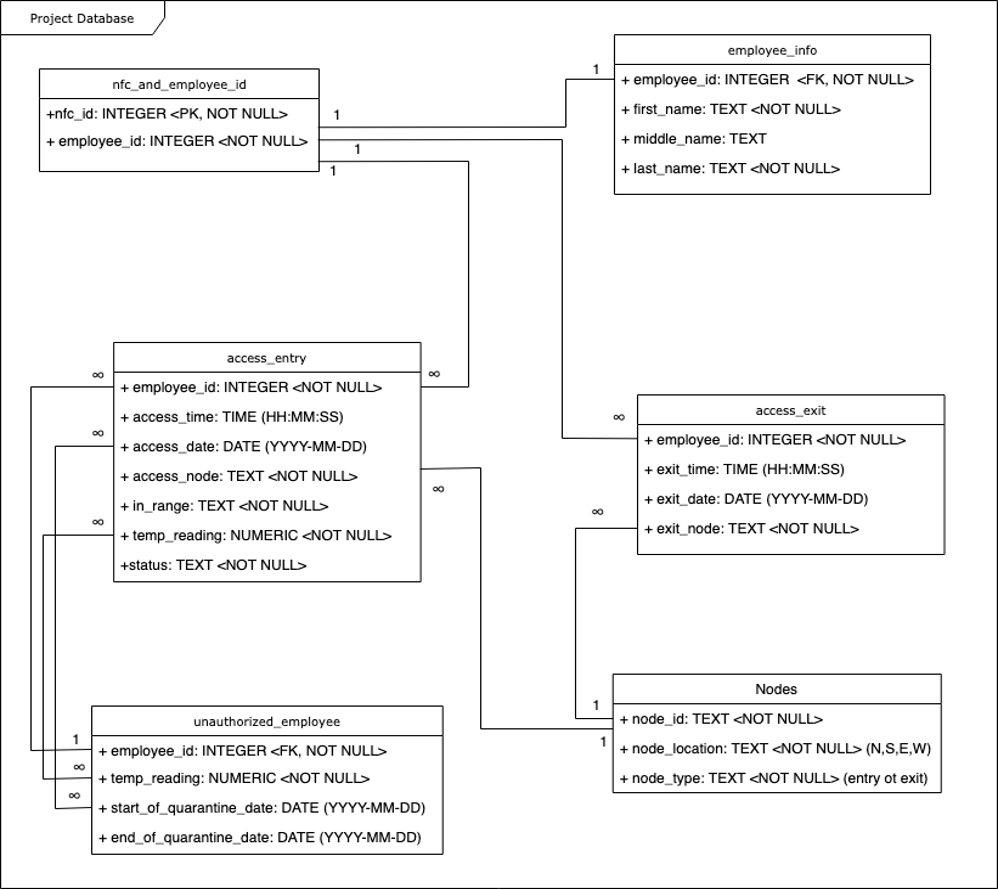
\includegraphics[width=\textwidth]{figures/db-schema.png}
\caption{Database Schema}
\end{figure}

